The previous section outlined the science case for a telescope on the lunar farside and the results are summarized in Appendix A.  Obviously ideally one would build a large and flexible observatory, and discussions for such telescopes are underway (see e.g. ).  However, in order to take advantage of the unique opportunity to take early measurements two additional constraints inform the design of the payload: (1) land and operate before the end of the decade (by 2030) and (2) achieve the goals for a budget at US\$150M or less.  The design therefore is structured under these additional objectives which puts the scope in the order of the NASA Commercial Lunar Payload Service (CLPS) program.  This scope is a lander of order 4m in span and 100 kg.  One difference from the CLPS program is the ability to work with potential vendors to address electromagnetic compatibility and radio frequency interference.  Table \ref{tab:constraints} summarizes the scope of the payload that fits within the constraints.

\begin{table}
    \caption{Payload Requirements}
    \begin{tabular}{|l|l|l|} \hline
    \textbf{Parameter} & \textbf{Value} & \textbf{Notes} \\ \hline
    \textbf{Span} & $\sim$4 m & This varies with vendor. \\ \hline
    \textbf{Mass} & 100 kg & This is the science payload mass. \\ \hline
    \textbf{Power (day)} & 100 W & Balancing day/night operations. \\ \hline
    \textbf{Power (night)} & 40 W & Included in the lander mass budget. \\ \hline
    \textbf{Comms} & 100 GB/month & The nominal budget includes 20 weeks of operation \\ \hline
    \textbf{Storage} & 20 TB & This coupled with comms and processing scopes the system. \\ \hline
    \end{tabular}
    \label{tab:constraints}
\end{table}

The science payload includes a mid-band phased array operating from 250--750 MHz, a wide band and high band antenna (750-2250 MHz), an ``FM'' band antenna (60--110 MHz), and a low band antenna (1--50 MHz). A schematic of the payload is shown in Figure \ref{fig:block}.

\begin{figure}
	\centering
	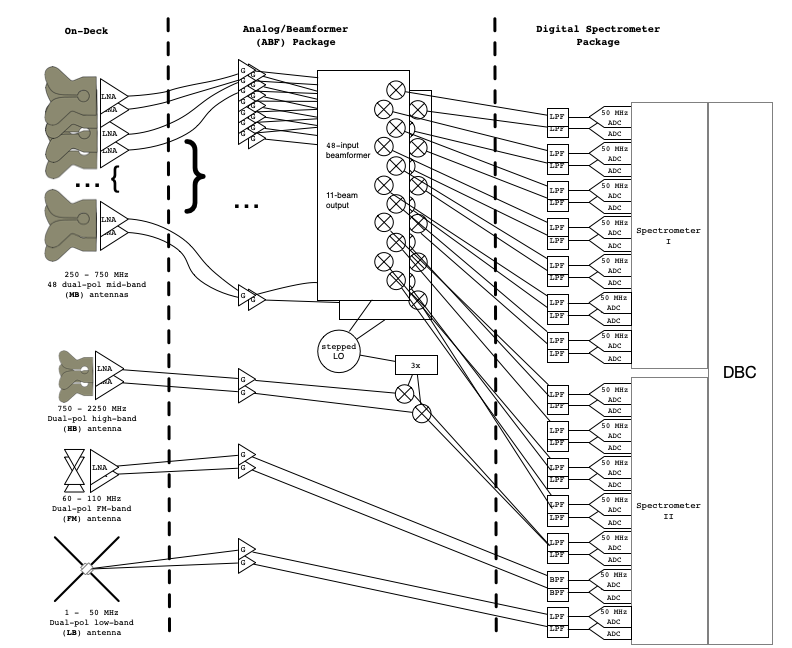
\includegraphics[width=\linewidth]{figures/SciencePayload.png}
	\caption{Block diagram of the science payload.\label{fig:block}}
\end{figure}

The mid-band array covers the bulk of the lander top surface with 48 dual polarizatio wideband antenna elements. The array forms a fan of beams on the sky designed to cover most of the lunar sky over time (Fig.\ \ref{fig:midband_beam_maps}). Formed beam output signals are downconverted and sampled in a 50 MHz subband that is scanned repeatedly across the array operating bandwidth. 

\begin{figure}
	\centering
	\includegraphics[width=\linewidth]{figures/midband_array_28cm_3dBSLL_beams_max.eps}
	\caption{Midband array formed beams over frequency. Scale is aperture efficiency in dB relative to a 3 meter diameter area. Beams are centered within 11 equal intervals over a 120 degree field of view.}
	\label{fig:midband_beam_maps}
\end{figure}


The operational constraints have a huge impact on the observing strategy, data products and download.  The full daytime available power is 100W, which reduces to 40W at night, and the expected download capacity is 100 GB/month.  The expected on-board memory will be between 10-20 TB.  The beamformer and individual antennas will produce dual-linear polarizations.  The spectrometer will have two main modes:
\begin{itemize}[noitemsep]
    \item Ring-buffer triggered baseband
    \item Pseudo-Stokes dynamic spectra of varying spectral/temporal resolution.
\end{itemize}

\subsection{Vehicle Lifespan and Programatics}
    As mentioned previously, the mission is targeted of launch in 2028. High level functional requirement for operations window is twenty weeks. With any aditional time and data intake is past considered mission requirements. Programatics sequence for the mission will follow a timeline as modeled. 
%\begin{itemize}
%    \item 
%\end{itemize}

\subsection{Calibration Logistics}
Calibration will take place through federated data approach. The landing system will process a landing location prior to comm system boot. Once the comm system is operational it will confirm and update the location and orientation. Imagery will also be secondary means of lander location confirmation. Contingency location confirmation may be used through NASA Laser reflectors. Measurments of exact beam outputs from orbiter and lander may also be used for calibration. 